\documentclass[11pt, a4paper]{article} % use larger type; default would be 10pt

\usepackage{fontspec} % Font selection for XeLaTeX; see fontspec.pdf for documentation
\defaultfontfeatures{Mapping=tex-text} % to support TeX conventions like ``---''
\usepackage{xunicode} % Unicode support for LaTeX character names (accents, European chars, etc)
\usepackage{xltxtra} % Extra customizations for XeLaTeX
\usepackage{tikz}
\usetikzlibrary{arrows,calc,patterns}


% other LaTeX packages.....
\usepackage{fullpage}
\usepackage[top=2cm, bottom=4.5cm, left=2.5cm, right=2.5cm]{geometry}
\usepackage{amsmath,amsthm,amsfonts,amssymb,amscd,systeme}
\usepackage{unicode-math}
\usepackage{cancel}
\geometry{a4paper} 
%\usepackage[parfill]{parskip} % Activate to begin paragraphs with an empty line rather than an indent
\usepackage{fancyhdr}
\usepackage{listings}
\usepackage{graphicx}
\usepackage{hyperref}
\usepackage{multicol}

% FONTS
% \setmainfont[Ligatures=TeX]{Cambria Math} % set the main body font (\textrm), assumes Charis SIL is installed
%\setsansfont{Deja Vu Sans}
% \setmonofont[Ligatures=TeX]{Fira Code}
\setmathfont[Ligatures=TeX]{NewCMMath-Regular}

\setmainfont{Cambria}
\setmonofont[Ligatures=TeX]{Roboto Mono}

\renewcommand\lstlistingname{Algorithm}
\renewcommand\lstlistlistingname{Algorithms}
\def\lstlistingautorefname{Alg.}
\lstdefinestyle{mystyle}{
    % backgroundcolor=\color{backcolour},   
    % commentstyle=\color{codegreen},
    % keywordstyle=\color{magenta},
    % numberstyle=\tiny\color{codegray},
    % stringstyle=\color{codepurple},
    basicstyle=\ttfamily\footnotesize,
    breakatwhitespace=false,         
    breaklines=true,                 
    captionpos=b,                    
    keepspaces=true,                 
    numbers=left,                    
    numbersep=5pt,                  
    showspaces=false,                
    showstringspaces=false,
    showtabs=false,                  
    tabsize=2
}
\lstset{style=mystyle}

\hypersetup{
  colorlinks   = true, %Colours links instead of ugly boxes
  urlcolor     = blue, %Colour for external hyperlinks
  linkcolor    = blue, %Colour of internal links
  citecolor   = red %Colour of citations
}


\newcommand\course{MS1 - Algebra}
\newcommand\hwnumber{Контрольна Робота 1}                   % <-- homework number
\newcommand\idgroup{111-2023}                
\newcommand\idname{Михайло Корешков}  

\usepackage[framemethod=TikZ]{mdframed}
\mdfsetup{%
	backgroundcolor = black!5,
}
\mdfdefinestyle{ans}{%
    backgroundcolor = green!5,
    linecolor = green!50,
    linewidth = 1pt,
}

\pagestyle{fancyplain}
\headheight 35pt
\lhead{\idgroup \\ \idname}
\chead{\textbf{\Large \hwnumber}}
\rhead{\course \\ \today}
\lfoot{}
\cfoot{}
\rfoot{\small\thepage}
\headsep 1.5em

\linespread{1.1}

\newcommand{\R}{\mathbb{R}}
\newcommand{\N}{\mathbb{N}}
\newcommand{\Z}{\mathbb{Z}}
\newcommand{\F}{\mathbb{F}}
\newcommand{\Q}{\mathbb{Q}}
\DeclareMathOperator{\lcm}{lcm}
\DeclareMathOperator{\cd}{CD}
\DeclareMathOperator{\ch}{char}
\DeclareMathOperator{\ob}{Ob}
\DeclareMathOperator{\mor}{Mor}
\DeclareMathOperator{\catring}{Ring}

\newtheorem*{proposition}{Твердження}
\newtheorem*{definition}{Визначення}

\begin{document}

\begin{mdframed}[backgroundcolor=pink!30]
    Варіант 3\\
    Завдання 1, 3.2, 4, 7, 8.1, 9.2, 10, 13, 14
\end{mdframed}

\subsection*{Ex 1}
\begin{mdframed}
    Довести
    \[(c\mid ab) \land (\gcd(a,c)=d) \implies c \mid db\]
\end{mdframed}

\begin{proof}
    \begin{gather*}
        \gcd(a,c)=d \implies \exists x,y\in\Z: ax + cy = d\\
        c\mid ab \implies \exists z\in\Z: ab = zc\\
        db = (ax+cy)b = (ab)x + cby = (zc)x + cby = c(zx+by)
    \end{gather*}
    Отримали, що $c \mid db$
\end{proof}

\subsection*{Ex 3.2}
\begin{mdframed}
    Знайти $\gcd$ та виразити його у вигляді лін комб $a,b$.
    $$a = 7854, \qquad b = 6960$$
\end{mdframed}
\begin{lstlisting}
    7854 = 1 * 6960 + 894
    6960 = 7 * 894 + 702
    894 = 1 * 702 + 192
    702 = 3 * 192 + 126
    192 = 1 * 126 + 66
    126 = 1 * 66 + 60
    66 = 1 * 60 + 6
    60 = 10 * 6 + 0
\end{lstlisting}
Останній ненульовий залишок - $6$, отже
\begin{mdframed}[style=yellow!20]
    $$\gcd(7854,6960) = 6$$
\end{mdframed}
Знайдемо лінійну комбінацію
\begin{lstlisting}
    7854 = a
    6960 = b
    894 = a-1*b = a-b 
    702 = b - 7(a-b) = -7a + 8b
    192 = 894 - 1 * 702 = a-b - (-7a + 8b) = 8a-9b
    126 = 702 - 3 * 192 = -7a + 8b - 3(8a-9b) = -31a+35b
    66 = 192 - 1 * 126 = 8a-9b - (-9a+35b) = 39a-44b
    60 = 126 - 1 * 66 = -31a+35b - (39a-44b) = -70a+79b
    6 = 66 - 60 = 39a-44b - (-70a+79b) = 109a-123b
\end{lstlisting}
Перевірка:
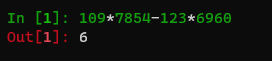
\includegraphics[width=0.5\textwidth]{gcd1.png}

Отже,
\begin{mdframed}[style=yellow!20]
    $$6 = 109\cdot 7854 - 123 \cdot 6960$$
\end{mdframed}

\subsection*{Ex 4}
\begin{mdframed}
    Довести
    \[([a]_n = [1]_n) \implies \gcd(a,n)=1\]
    Показати контрприклад для оберненого твердження
\end{mdframed}

\begin{proof}
    $$([a]_n = [1]_n)  \implies n\mid (a-1) \implies \exists k\in\Z: (a-1)=nk$$
    $$a-nk=1$$
    $$ax+ny=1, \quad x=1, y=-k$$
    Знайшли лінійну комбінацію $a,n$ що дає $1$. З цього, $\gcd(a,n)=1$
\end{proof}
Покажемо контрприклад для оберненого твердження.
$$a = 7, n = 5, [a]_n = [2]_n\ne [1]_n, \gcd(a,n)=1$$


\subsection*{Ex 7}
\begin{mdframed}
    Нехай $a,b\in\Z$. Нехай $P=\{2,3,5,7,11,...\}$ - множина додатніх незвідних цілих чисел.
    Довести:
    \[\left(\forall q\in P: a = b \mod q\right) \implies a=b\]
\end{mdframed}

\begin{proof}
    Нехай $g = \gcd(a,b)$.
    Тоді 
    \begin{gather*}
        a = gx\\
        b = gy\\
        \gcd(x,y) = 1
    \end{gather*}
    Далі
    \begin{gather*}
        \forall q\in P: a-b = qk \\
        gx-gy = g(x-y) = qk \\
        \forall q\in P: q \mid g(x-y) \\
    \end{gather*}

    Єдине таке число, яке ділиться на всі прості числа, це $0$.
    Тобто $g(x-y) = 0$
    \[
    \left[\begin{matrix}
        g = 0 &\implies& a=b=0\\
        (x-y)=0 &\implies& x=y \implies a=b
    \end{matrix}\right.
    \]

    Отже, $a=b$.
\end{proof}

\newpage
\subsection*{Ex 8.1}
\begin{mdframed}
    Розв'язати
    \[\begin{cases}
        x \equiv 1 \mod 25\\
        3x \equiv 2 \mod 27\\
        x \equiv 13 \mod 59\\
    \end{cases}\]
\end{mdframed}

По-перше, позбавляємось коефіцієнтів при $x$.

$$3x \equiv 2 \mod 27$$
Зверну увагу, що $3\mid 27$, але $3\nmid 2$. Тоді це рівняння не має розв'язків.

А тоді вся система рівнянь не має розв'язків.

\subsection*{Ex 9.2}
\begin{mdframed}
    Обчислити $34^{56789} \mod 13$
\end{mdframed}

Зверну увагу, що $\gcd(13,34)=\gcd(13,10)=1$, 13 - просте.

\[34^{56789} \equiv 8^{56789}\]
\[8^2 \equiv 12 \equiv (-1) \mod 13\]
\[8^4 \equiv 12^2 \equiv 14 \equiv 1 \mod 13\]
\[8^{56789} = 8^{56788+1} = 8^{4k}\cdot 8^1 = 1\cdot 8 = 8\]

Інакшим способом,

\begin{lstlisting}
    56789 = 4368*13 + 5
    4368 = 336*13 + 0
    336 = 25*13 + 11
    25 = 1*13 + 12
\end{lstlisting}
Таким чином
\[56789 = 1\cdot 13^4 + 12\cdot 13^3 + 11\cdot 13^2 + 5\]
З цього
\[8^{56789} \equiv 8^{1+12+11+5} \equiv 8^{29} \equiv 8^{2\cdot 13 + 3} \equiv 8^{5} \mod 13\]
\[8^{5} \equiv 64\cdot 64 \cdot 8 \equiv (-1) \cdot (-1) \cdot 8 = 8 \mod 13\]

Отже,
\begin{mdframed}[backgroundcolor=yellow!20]
    $$34^{56789} \equiv 8 \mod 13$$
\end{mdframed}

\newpage
\subsection*{Ex 10}
\begin{mdframed}
    $R$ - область цілісності.\\
    Довести, що $\ch R$ - просте.
\end{mdframed}

$\ch R = \begin{cases}
    \min \{k\in\N \mid k\cdot 1_R = 0_R\}, & \exists k: k\cdot 1_R = 0_R\\
    0, & \text{otherwise}
\end{cases} $

$R$ - область цілісності якщо $R$ - ненульове комутативне кільце без дільників нуля (окрім нуля).
Тобто
\[\forall a,b\in R: (ab=0) \implies (a=0) \vee (b=0)\]

\begin{proof}
    Нехай $1_R \ne 0_R$. \\
    Припустимо, що $\ch R = n$ - не просте. 
    Тобто $\exists k,l>1: n = kl$.\\
    Нехай $a = k\cdot 1_R, \quad b = l\cdot 1_R$.
    Також зверну увагу, що $k,l < n$.\\
    Оскільки $n$ - найменше число таке, що $n\cdot 1_R=0_R$, $a\ne 0_R, b\ne 0_R$.

    Розглянемо добуток $ab$
    \[ab = (k\cdot 1_R) \cdot (l \cdot 1_R) = (\underset{k}{\underbrace{1+1+\cdots+1}}) \cdot (\underset{l}{\underbrace{1+1+\cdots+1}}) = \]
    \[= \left(\underset{k}{\underbrace{(\underset{l}{\underbrace{1+1+\cdots+1}}) + (\underset{l}{\underbrace{1+1+\cdots+1}}) + \cdots + (\underset{l}{\underbrace{1+1+\cdots+1}})}}\right) = \]
    \[= \underset{kl}{\underbrace{1+1+\cdots+1}} = n\cdot 1_R = 0_R\]
    Що суперечить тому, що $R$ - область цілісності, адже $a\ne0_R, b\ne0_R$.

    Таким чином довели, що $n$ - просте.
\end{proof}

\newpage
\subsection*{Ex 13}
\begin{mdframed}
    $S = \{[0]_6, [3]_6\} \subset \Z/6\Z$\\
    Відомо, що $S$ замкнена відносно операцій.
    \begin{enumerate}
        \item Чи є $S$ кільцем?
        \item Чи є $S$ підкільцем $R$?
    \end{enumerate}
\end{mdframed}

\subsection*{а) Чи є $S$ кільцем?}
\begin{enumerate}
    \item Коректність операцій - ОК
    \item Асоціативність - ОК
    \item Нуль: $O_S = O_R = [0]_6$
    \item Обернені відносно додавання: $[3]_6+[3]_6=[6]_6=[0]_6$ - ОК
    \item Комутативність додавання - ОК
    \item Асоціативність множення - ОК
    \item Одиниця: $[0]_6\cdot [3]_6 = 0, [3]_6\cdot [3]_6 = [9]_6 = [3]_6$
    \[1_S = [3]_6\]
    \item Дистрибутивність - ОК
\end{enumerate}
Отже, $S$ є кільцем

\subsection*{б) Чи є $S$ підкільцем $R$?}
Ні, $S$ не є підкільцем, бо $1_R = [1]_6 \notin S$, $1_R \ne 1_S$.


\subsection*{Ex 14}
\begin{mdframed}
    Нехай $R,S$ - кільця. Нехай $f: R \to S$ - сюр'єктивне відображення, що зберігає операції.
    Тобто
    \[\begin{cases}
        f(a+b) = f(a) + f(b),\\
        f(ab) = f(a)f(b)
    \end{cases}\]
    Довести, що $f(1_R)=1_S$, тобто $f$ - гомоморфізм кілець.
\end{mdframed}
\begin{proof}
    Спершу,
    \[\forall b \in S: \exists f^{-1}(b)=a \in R\]
    Тоді 
    \[\forall b\in S: b\cdot f(1_R) = f(f^{-1}(b))\cdot f(1_R) = f(f^{-1}(b) \cdot 1_R) = f(f^{-1}(b)) = b  \]
    \[\forall b\in S: f(1_R)\cdot b = f(1_R)\cdot f(f^{-1}(b))  = f(1_R \cdot f^{-1}(b)) = f(f^{-1}(b)) = b  \]
    Тобто, довели, що $f(1_R)$ - дійсно одиниця в $S$. 

    Таким чином довели, що $f$ - гомоморфізм кілець.
\end{proof}



\end{document}

